\documentclass{beamer}
\usepackage[utf8]{inputenc}
\usepackage[T1]{fontenc}
\usepackage[ngerman]{babel}
\usepackage{ae}
\usepackage{array}
\usepackage{tabularx}
\usepackage{graphicx}
\usepackage{amsmath}
\usepackage{textcomp}
\usepackage{blindtext}
\usepackage{listings}
\usepackage{booktabs}
\usepackage{icomma}

%Settings
\usepackage{icomma}

%Beamer Einstellungen
\usetheme{Goettingen}
\newcounter{chapter}

\setbeamertemplate{section in head/foot}{\hfill\thechapter.\insertsectionheadnumber.~\insertsectionhead}
\setbeamertemplate{section in head/foot shaded}{\color{structure!50}\hfill\thechapter.\insertsectionheadnumber.~\insertsectionhead}
\setbeamertemplate{section in toc}{\large\thechapter.\inserttocsectionnumber~\inserttocsection}
\makeatletter
\setbeamertemplate{section in sidebar}%{sidebar theme}
{%
  \vbox{%
    \vskip1ex%
    \beamer@sidebarformat{3pt}{section in sidebar}{\thechapter.\insertsectionheadnumber
~\insertsectionhead}%
  }%
}
\setbeamertemplate{section in sidebar shaded}%{sidebar theme}
{%
  \vbox{%
    \vskip1ex%
    \beamer@sidebarformat{3pt}{section in sidebar shaded}{\thechapter.\insertsectionheadnumber
~\insertsectionhead}%
  }%
}
\addtobeamertemplate{navigation symbols}{%
	\usebeamerfont{footline}%
 	\usebeamercolor[fg]{footline}%
 	\raisebox{.25ex}{\insertframenumber/\inserttotalframenumber}
}{}
\makeatother

%Farbe
\definecolor{mygreen}{rgb}{0,0.6,0}
\definecolor{mygray}{rgb}{0.5,0.5,0.5}
\definecolor{mymauve}{rgb}{0.58,0,0.82}
\definecolor{mybygrey}{gray}{.93}
\definecolor{eclipse-comments}{rgb}{0,0.6,0}
\definecolor{eclipse-strings}{rgb}{1,0,1}
\definecolor{eclipse-keywords}{rgb}{0,0,1}

% Lenghts
\setlength{\parskip}{.5\baselineskip plus .2\baselineskip minus .1\baselineskip}

%Eurozeichen
\usepackage{eurosym}
\DeclareUnicodeCharacter{20AC}{\euro}

%tabellen
\newcolumntype{L}{>{\raggedright\arraybackslash}X}

%Listings Ilog-Script-Definition
\lstdefinelanguage{IlogScript}{
  keywords=[1]{typeof, new, true, false, catch, function, return, null, catch, switch, var, if, in, while, do, else, case, break, for},
  keywordstyle=[1]\color{orange}\bfseries,
  keywords=[2]{class, export, boolean, throw, implements, import, this, execute, int, main},
  keywordstyle=[2]\color{blue}\bfseries,
  keywords=[3]{write, writeln, thisOplModel, cplex},
  keywordstyle=[3]\color{RedViolet}\bfseries,
  identifierstyle=\color{black},
  sensitive=false,
  comment=[l][\color{eclipse-comments}]{//},%
  morecomment=[s]{/*}{*/},
  commentstyle=\color{purple}\ttfamily,
  stringstyle=\color{mymauve}\ttfamily,
  morestring=[b]',
  morestring=[b]",
  showstringspaces=false
}[keywords,comments,strings]%

%Listings OPL Definition
\lstdefinelanguage[]{opl}%
{
  keywords=[1]{
    maximize, minimize, subject, to, forall, sum, solve, string, dvar, boolean, int, int+, float, float+, enum, tupel, ftoi, mod, abs, maxint, sqrt, ceil, floor, distToInt, frac, trunc, infinity, first, last, card, ord, next, prev, range, in, struct, prod, min, max, union, inter, not, initialize, var, dmin, dmax, dsize, bound, dnexthigher, alldifferent, circuit, distribute, try, endtry, tryall, if, endif, then, else, while, select, once, search, when, onValue, generate, generationMin, generationMax, generateSeq
  },
  keywordstyle=[1]\color{eclipse-keywords},
  morekeywords={..,=,<,>,<=,=>,==},
  keywords=[2]{typeof, new, true, false, catch, function, return, null, catch, switch, var, if, in, while, do, else, case, break},
  keywordstyle=[2]\color{orange}\bfseries,
  keywords=[3]{write, writeln, thisOplModel, from, DBConnection, DBRead, DBUpdate, SheetConnection, SheetRead, SheetWrite},
  keywordstyle=[3]\color{RedViolet}\bfseries,
  comment=[l][\color{eclipse-comments}]{//},%
  morecomment=[s][\color{eclipse-comments}]{/*}{*/},%
  string=[b][\color{eclipse-strings}]\``,%
  stringstyle=\color{mymauve}\ttfamily,
  morestring=[b]",%
  morestring=[b]',%
  showstringspaces=false
}[keywords,comments,strings]%

\lstset{ %
  backgroundcolor=\color{mybygrey},   % choose the background color; you must add \usepackage{color} or \usepackage{xcolor}
  basicstyle=\footnotesize\ttfamily,
  captionpos=b,                    % sets the caption-position to bottom
  commentstyle=\color{mygreen},    % comment style
  %deletekeywords={...},            % if you want to delete keywords from the given language
  escapeinside={\%*}{*)},          % if you want to add LaTeX within your code
  frame=leftline,                    % adds a frame around the code
  keywordstyle=\color{blue},       % keyword style
  language=opl,                 % the language of the code
  linewidth=\textwidth,
  morekeywords={*,documentclass,begin,title,author,date,maketitle},            % if you want to add more keywords to the set
  numbers=left,                    % where to put the line-numbers; possible values are (none, left, right)
  numbersep=5pt,                   % how far the line-numbers are from the code
  numberstyle=\tiny\color{mygray}, % the style that is used for the line-numbers
  rulecolor=\color{black},         % if not set, the frame-color may be changed on line-breaks within not-black text (e.g. comments (green here))
  stepnumber=1,                    % the step between two line-numbers. If it's 1, each line will be numbered
  stringstyle=\color{mymauve},     % string literal style
  tabsize=2,                       % sets default tabsize to 2 spaces
  xleftmargin=.05\textwidth,
  literate=%
    {Ö}{{\"O}}1
    {Ä}{{\"A}}1
    {Ü}{{\"U}}1
    {ß}{{\ss}}1
    {ü}{{\"u}}1
    {ä}{{\"a}}1
    {ö}{{\"o}}1
    {~}{{\textasciitilde}}1,
  title=\lstname                   % show the filename of files included with \lstinputlisting; also try caption instead of title
}

%Listings OPL Data Definition
\lstdefinelanguage[]{opldata}%
{
  keywords=[1]{
    maximize, minimize, subject, forall, sum, solve, string, dvar, boolean, int, int+, float, float+, enum, tupel, ftoi, mod, abs, maxint, sqrt, ceil, floor, distToInt, frac, trunc, infinity, first, last, card, ord, next, prev, range, in, struct, prod, min, max, union, inter, not, initialize, var, dmin, dmax, dsize, bound, dnexthigher, alldifferent, circuit, distribute, try, endtry, tryall, if, endif, then, else, while, select, once, search, when, onValue, generate, generationMin, generationMax, generateSeq
  },
  keywordstyle=[1]\color{eclipse-keywords},
  morekeywords={..,=,<,>,<=,=>,==},
  keywords=[2]{typeof, new, true, false, catch, function, return, null, catch, switch, var, if, in, while, do, else, case, break},
  keywordstyle=[2]\color{orange}\bfseries,
  keywords=[3]{write, writeln, thisOplModel, from, to, DBConnection, DBRead, DBUpdate, SheetConnection, SheetRead, SheetWrite},
  keywordstyle=[3]\color{RedViolet}\bfseries,
  comment=[l][\color{eclipse-comments}]{//},%
  morecomment=[s][\color{eclipse-comments}]{/*}{*/},%
  string=[b][\color{eclipse-strings}]\``,%
  stringstyle=\color{mymauve}\ttfamily,
  morestring=[b]",%
  morestring=[b]',%
  showstringspaces=false
}[keywords,comments,strings]%

\lstset{ %
  backgroundcolor=\color{mybygrey},   % choose the background color; you must add \usepackage{color} or \usepackage{xcolor}
  basicstyle=\footnotesize\ttfamily,
  captionpos=b,                    % sets the caption-position to bottom
  commentstyle=\color{mygreen},    % comment style
  %deletekeywords={...},            % if you want to delete keywords from the given language
  escapeinside={\%*}{*)},          % if you want to add LaTeX within your code
  frame=leftline,                    % adds a frame around the code
  keywordstyle=\color{blue},       % keyword style
  language=opl,                 % the language of the code
  linewidth=\textwidth,
  morekeywords={*,documentclass,begin,title,author,date,maketitle},            % if you want to add more keywords to the set
  numbers=left,                    % where to put the line-numbers; possible values are (none, left, right)
  numbersep=5pt,                   % how far the line-numbers are from the code
  numberstyle=\tiny\color{mygray}, % the style that is used for the line-numbers
  rulecolor=\color{black},         % if not set, the frame-color may be changed on line-breaks within not-black text (e.g. comments (green here))
  stepnumber=1,                    % the step between two line-numbers. If it's 1, each line will be numbered
  stringstyle=\color{mymauve},     % string literal style
  tabsize=2,                       % sets default tabsize to 2 spaces
  xleftmargin=.05\textwidth,
  literate=%
    {Ö}{{\"O}}1
    {Ä}{{\"A}}1
    {Ü}{{\"U}}1
    {ß}{{\ss}}1
    {ü}{{\"u}}1
    {ä}{{\"a}}1
    {ö}{{\"o}}1
    {~}{{\textasciitilde}}1,
  title=\lstname                   % show the filename of files included with \lstinputlisting; also try caption instead of title
}

% Makros
\RequirePackage{ifthen}
\newcommand{\sectionframe}[2][\empty]{
  \ifthenelse{\equal{#1}{\empty}}
    {\section{#2}}
    {\section[#1]{#2}}
  \begin{frame}
   \begin{center}
    \LARGE\bfseries \thechapter.\thesection{} #2
   \end{center}
  \end{frame}
}

\newcommand{\subsectionframe}[2][\empty]{
  \ifthenelse{\equal{#1}{\empty}}
    {\subsection{#2}}
    {\subsection[#1]{#2}}
  \begin{frame}
   \begin{center}
    \Large\bfseries #2
   \end{center}
  \end{frame}
}



%Always load hyperref last...
\usepackage{hyperref}


\begin{document}

\setcounter{chapter}{5}
\author[CC-BY-SA A.~Popp]{Andreas Popp\vspace{-2\baselineskip}}
\date[CC-BY-SA]{\begin{center}
                 
\includegraphics[width=.2\linewidth]{Icons/CCBYSAbig}
                \end{center}
\footnotesize Dieser Foliensatz ist lizenziert unter einer  \href{http://creativecommons.org/licenses/by-sa/4.0/}{Creative Commons Namensnennung - Weitergabe unter gleichen Bedingungen 4.0 International Lizenz}.}
\title[\thechapter{} Probleme mit mehreren Zielfunktionen]{\textbf{Modellierung und Optimierung mit OPL}\newline \thechapter{} Probleme mit mehreren Zielfunktionen}

\frame{\titlepage}


\begin{frame}[squeeze]
 \frametitle{Inhalt}\scriptsize
  \tableofcontents
\end{frame}

\begin{frame}
 \frametitle{Example: Vindoo Support}
 \begin{figure}
  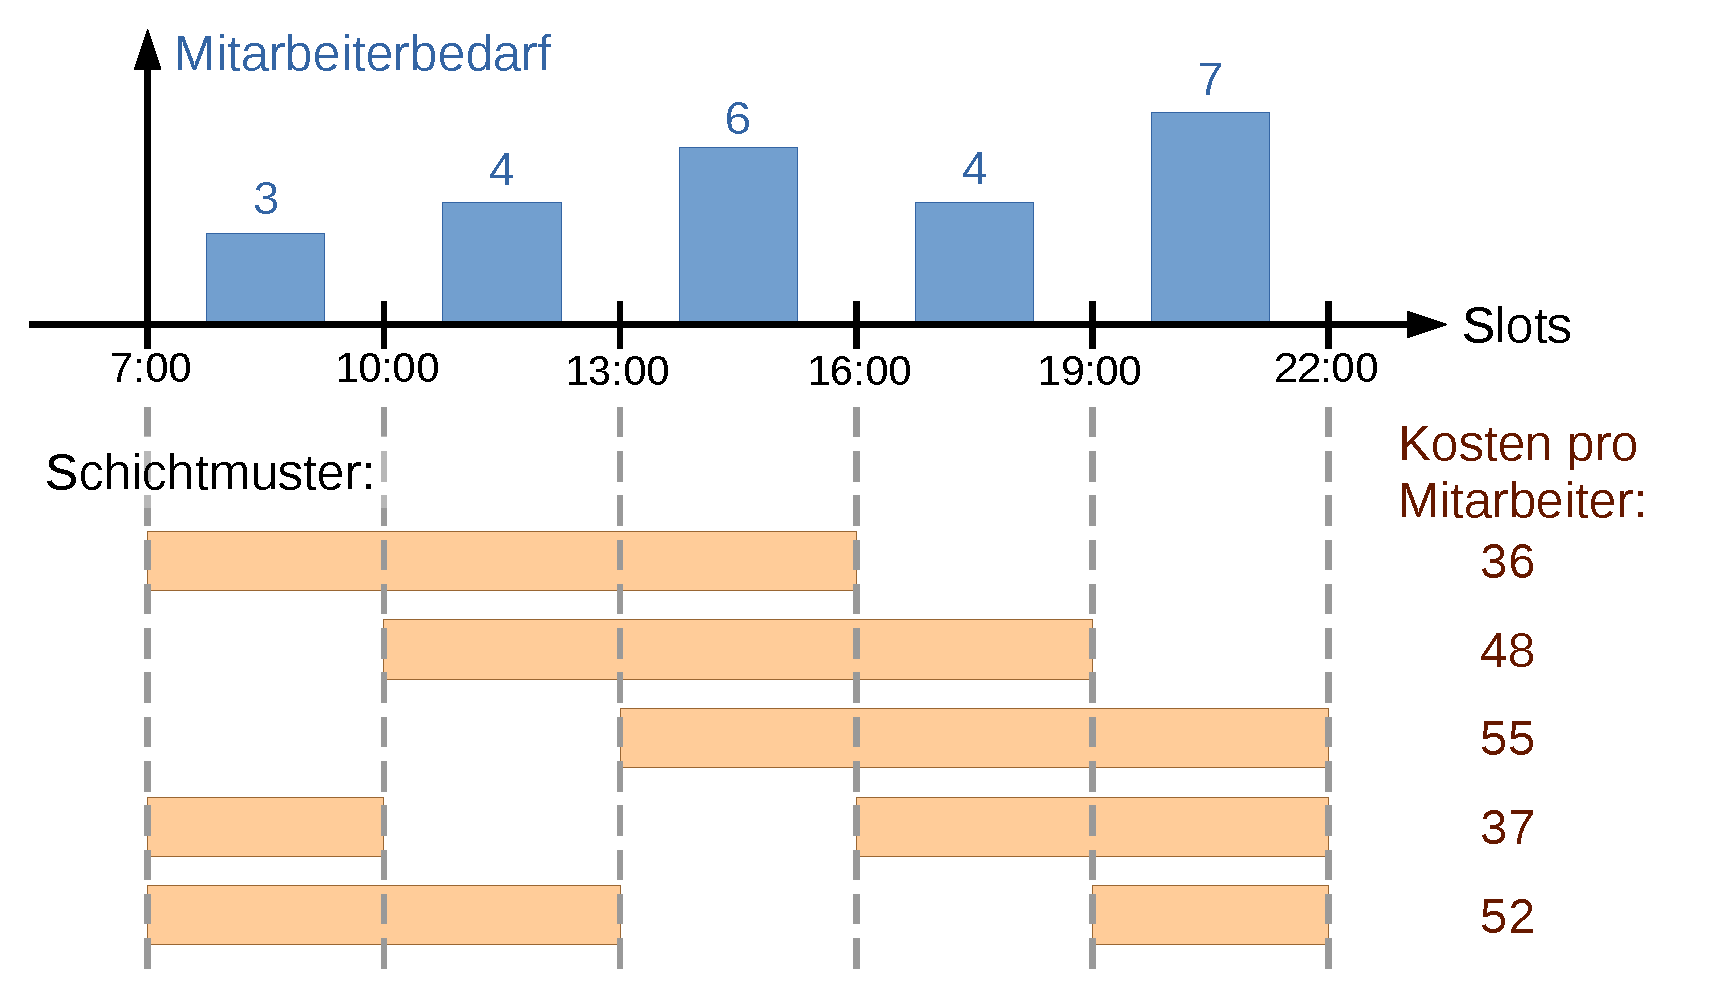
\includegraphics[width=\linewidth]{Bilder/Vindoo}
 \end{figure}
 {\footnotesize(cf. Pinedo: Planning and Scheduling in Manufacturing and Services)}
\end{frame}

\begin{frame}
 \frametitle{Model: Cyclic staffing problem}
 \begin{tabularx}{\linewidth}{lL}
  \multicolumn{2}{l}{\textbf{index sets}:}\\
     $T$ & set of time slots\\
     $S$ & set of shift patterns\\
  \multicolumn{2}{l}{\textbf{parameters}:}\\
     $c_s$ & cost per employee in shift pattern~$s\in S$\\
     $d_t$ & requirement of employees in shift pattern~$t\in T$\\
     $a_{ts}$ & Availability of employees in shift pattern~$s\in S$ in time slot~$t\in T$\\
  \multicolumn{2}{l}{\textbf{decision variables}:}\\
     $x_s$ & deployed employees in shift pattern~$s\in S$\\[1ex]
  \multicolumn{2}{l}{\textbf{model description}:}\\[1ex]
  \multicolumn{2}{l}{
      $
      \begin{array}{rllr}
	\min & \multicolumn{3}{l}{
		  \displaystyle\sum_{s\in S}c_s\cdot x_s
		}\\[3ex]
	s.t. & \displaystyle\sum_{s\in S} a_{ts}\cdot x_s \geq d_t & \quad\forall t\in T  & \mathrm{(I)}\\[.8ex]
	      & x_s \in\mathbb{Z}_0^+ & \quad\forall s\in S &\\
      \end{array}
      $
  }\\[1ex]
 \end{tabularx}
\end{frame}

\sectionframe[Optimization routine in OPL]{Optimization routine in OPL}
\begin{frame}
 \frametitle{Optimization routine in OPL}
 \begin{figure}
   \centering
   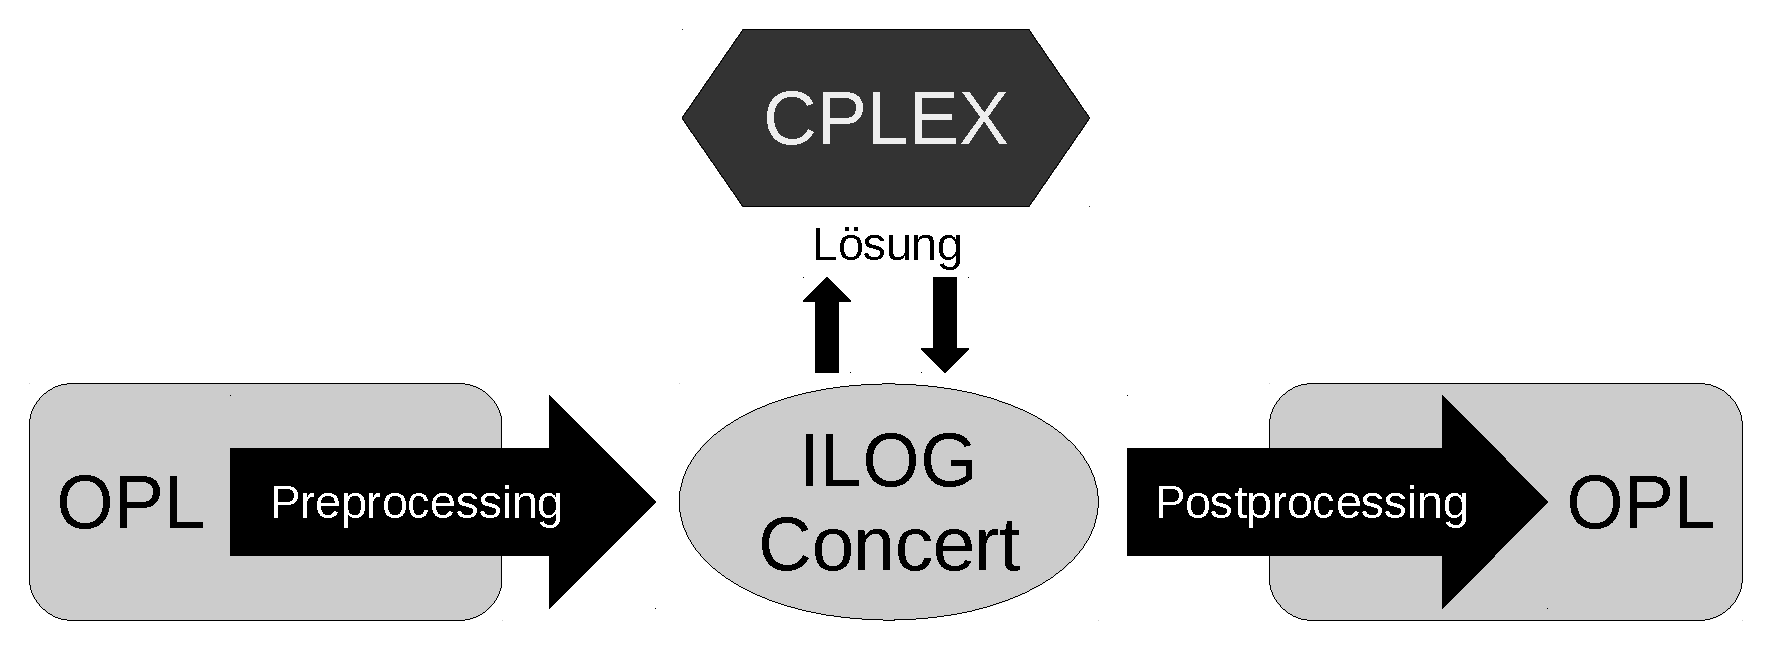
\includegraphics[width=\linewidth]{Bilder/OPL-Ablauf}
 \end{figure}
\end{frame}


\sectionframe{Linear Optimization}
\subsection{Properties}
\begin{frame}\small
 \frametitle{Linear functions and constraints}
 \begin{block}{Linear functions}
  \vspace{-2\baselineskip}
  \begin{equation*}
    f(x_1, \ldots, x_N) = \sum_{n=1}^{N} c_n\cdot x_n
  \end{equation*}
 \end{block}
 \vspace{-\baselineskip}
 \begin{block}{Linear constraints}
  Let $f$ be a linear function:
  \begin{align*}
   &f(x_1, \ldots, x_N) = b\\
   &f(x_1, \ldots, x_N) \leq b\\
   &f(x_1, \ldots, x_N) \geq b\\
  \end{align*}
 \end{block}
 \vspace{-2\baselineskip}
 \begin{block}{Linear optimization model}
  objective function and constraints linear in the decision variables $\Longrightarrow$ linear optimization model 
 \end{block}
\end{frame}

\begin{frame}
 \frametitle{Properties of linear functions}
 \begin{description}
  \item[Proportionality] Each variable contributes a proportional value to the function.
  \item[Independence] The value each variable contributes to the function is independent of the manifestation of the other variables.
 \end{description}
\end{frame}


\begin{frame}
 \frametitle{Typical signs for non-linearity}
 \begin{itemize}
  \item variables have other exponents than~$1$
  \begin{itemize}
   \item other natural exponents, e.g.: $x^2$
   \item roots, e.g.: $\sqrt{x} = x^{\frac{1}{2}}$
   \item variables in the denominator, e.g.: $\frac{1}{x} = x^{-1}$
  \end{itemize}
  \item variables are multiplied with each other, e.g.: $x_1\cdot x_2$
  \item exponential functions, e.g.: $2^x$
  \item absolute values, e.g. $|x|$
 \end{itemize}

 \begin{block}{Anomaly: constants}
  While constants are non-linear by definition, they do not interfere with linear optimization models, since they can be eliminated easily.
 \end{block}
\end{frame}

\begin{frame}
 \frametitle{deterministic vs. stochastic optimization models}
 \begin{description}
  \item[deterministic optimization models:] all parameters and function values are always exactly known
  \item[stochastic optimization models:] parameters and function values are subject to random deviations
 \end{description}
 
 Linear optimization models are deterministic in general.
\end{frame}

\begin{frame}
 \frametitle{continuous vs. integer optimization models}
 \begin{description}
  \item[continuous optimization models:] the values of the decision variables are continuous (real) values
  \item[integer optimization models:] the values of the decision variables can only be integer
 \end{description}
 
 \begin{block}{Types of linear optimization models by possible values for decision variables:}
  \begin{itemize}\footnotesize
   \item continuous decision variables $\Longrightarrow$ (continuous) linear optimization model
   \item integer decision variables $\Longrightarrow$ integer linear optimization model
   \item continuous and integer decision variables $\Longrightarrow$ mixed integer linear optimization model
  \end{itemize}
 \end{block}
\end{frame}

\subsection{Solution of linear problems}

\begin{frame}
 \frametitle{Solution structure of linear optimization models}
 Possible structure of solutions:
 \begin{itemize}
  \item there is exactly one optimal solution
  \item there is an unlimited number of optimal solutions
  \item there is no optimal solution
  \begin{itemize}
   \item the solution space is empty
   \item the solution space is unbound and the objective function approaches infinity
  \end{itemize}
 \end{itemize}
\end{frame}


\begin{frame}
 \frametitle{Well known solution methods for linear optimization models}
 \begin{block}{Solution methods for (continuous) linear optimization models}
  \begin{itemize}
    \item Dantzig's simplex method
    \item Karmarkar's inner point method
  \end{itemize}
 \end{block}
 \begin{block}{Solution methods for (mixed) integer linear optimization models}
  \begin{itemize}
    \item Branch and bound method
    \item Cutting planes methods
  \end{itemize}
 \end{block}
\end{frame}





\sectionframe{Modell und Modellinstanz}
\begin{frame}
 \frametitle{Optimierungsmodell aus Beispiel ``Lewig Sanstetten''}
 \begin{block}{Modell: Produktionsproblem}
 \Large
 \begin{equation*}
  \begin{array}{ll}
    \max & 2,9\cdot x_1 + 3,3\cdot x_2 + 2,2\cdot x_3\\
    s.t. & 5,3\cdot x_1 + 2,9\cdot x_2 + 2,5\cdot x_3 \leq 64\\
	  & 3,9\cdot x_1 + 4,8\cdot x_2 + 3,1\cdot x_3 \leq 48\\
	  & x_1\geq0,\,x_2\geq0,\,x_3\geq0\\
  \end{array}
 \end{equation*}
 \end{block}
\end{frame}

\begin{frame}
 \frametitle{Ersetzen von Daten durch Parameter (Formvariablen)}
 \begin{block}{Modell: Produktionsproblem}
 \Large
 \begin{equation*}
  \begin{array}{ll}
  \max & p_1\cdot x_1 + p_2\cdot x_2 + p_3\cdot x_3\\
  s.t. & v_{A1}\cdot x_1 + v_{A2}\cdot x_2 + v_{A3}\cdot x_3 \leq c_A\\
	& v_{B1}\cdot x_1 + v_{B2}\cdot x_2 + v_{B3}\cdot x_3 \leq c_B\\
	& x_1\geq0,\,x_2\geq0,\,x_3\geq0\\
  \end{array}
 \end{equation*}
 \end{block}
\end{frame}

\begin{frame}
 \frametitle{Indexmengen als spezielle Parameter}
 \begin{block}{Variante 1: Maximalindex als Parameter}
  Sei $I\in\mathbb{N}$ die Anzahl der Produkte, dann lautet zum Beispiel die Zielfunktion:
  \[
   \sum_{i=1}^I p_i \cdot x_i
  \]
 \end{block}
 \begin{block}{Variante 2: Indexmenge als Parameter}
  Sei $I$ die Menge der Produkte, dann lautet zum Beispiel die Zielfunktion:
  \[
   \sum_{i\in I} p_i\cdot x_i
  \]
 \end{block}
\end{frame}

\begin{frame}
 \frametitle{Summation über parametrisierte Indexmengen}
 \begin{block}{Modell: Produktionsproblem}
 \Large
 \begin{equation*}
  \begin{array}{ll}
  \max & \displaystyle\sum_{i\in I} p_i\cdot x_i\\
  s.t. & \displaystyle\sum_{i\in I} v_{Ai}\cdot x_i \leq c_A\\
	& \displaystyle\sum_{i\in I} v_{Bi}\cdot x_i \leq c_B\\
	& x_1\geq0,\,x_2\geq0,\,x_3\geq0\\
  \end{array}
 \end{equation*}
 \end{block}
\end{frame}

\begin{frame}
 \frametitle{Verwendung des Allquantors}
 \Large
 \begin{align*}
  & \sum_{i\in I} v_{Ai}\cdot x_i \leq c_A\\
  & \sum_{i\in I} v_{Bi}\cdot x_i \leq c_B
 \end{align*}
 \begin{center}\normalsize
  \structure{\textdownarrow{} Indexmenge $R$ der Ressourcen \textdownarrow{}}
 \end{center}
 \begin{equation*}
  \sum_{i\in I} v_{ri}\cdot x_i \leq c_r\qquad\alert{\forall r\in R}
 \end{equation*}
\end{frame}

\begin{frame}
 \frametitle{Allgemeines Modell}
 \begin{block}{Modell: Produktionsproblem}
 \begin{equation*}
  \begin{array}{lll}
  \max & \displaystyle\sum_{i\in I} p_i\cdot x_i\\
  s.t. & \displaystyle\sum_{i\in I} v_{ri}\cdot x_i \leq c_r&\qquad\forall r\in R \\
	& x_i\geq0 &\qquad\forall i\in I\\
  \end{array}
 \end{equation*}
 \end{block}
\end{frame}

\begin{frame}
 \frametitle{Modell: Produktionsproblem}
 \footnotesize
 \begin{tabularx}{\linewidth}{lL}
  \multicolumn{2}{l}{\textbf{Indexmengen}:}\\
   $I$& Menge der Produkte\\
   $R$& Menge der Ressourcen\\[1ex]
  \multicolumn{2}{l}{\textbf{Parameter}:}\\
   $p_i$& Preis von Produkt $i\in I$\\
   $c_r$& Kapazität von Ressource $r\in R$\\
   $v_{ri}$& Kapazitätsverbrauch von Produkt $i\in I$ auf Ressource $r\in R$\\[1ex]
  \multicolumn{2}{l}{\textbf{Entscheidungsvariablen}:}\\
   $x_i$& Produktionsmenge von Produkt $i\in I$\\[1ex]
  \multicolumn{2}{l}{\textbf{Modellbeschreibung}:}\\[1ex]
  \multicolumn{2}{l}{
      $
      \begin{array}{rllr}
	\max & \displaystyle\sum_{i\in I} p_i\cdot x_i & & \\[3ex]
	s.t. & \displaystyle\sum_{i\in I} v_{ri}\cdot x_i \leq c_r & \quad\forall r\in R & \mathrm{(I)}\\
		& x_i \geq 0 & \quad\forall i\in I & \\
      \end{array}
      $
  }
 \end{tabularx}
\end{frame}

\begin{frame}
 \frametitle{Modell vs. Modellinstanz}
 \begin{block}{Modell}
  Die \alert{allgemeine} Darstellung der Problemstruktur mit \alert{allgemeinen} Indexmengen und Parametern.
 \end{block}
 \begin{block}{Modellinstanz}
  Ein \alert{konkretes} Problem, in welchem den Indexmengen und Parametern \alert{konkrete} Werte zugewiesen wurden.
 \end{block}
\end{frame}

\sectionframe{Multicriteria optimization}
\begin{frame}
 Objective function as in example ``Lewbrandt GmbH'':
 \frametitle{Example objective function}
 \begin{itemize}
  \item Profit: $\max f_G(\mathbf{\overline{x}}) = 150\cdot x_1 + 100\cdot x_2 + 150\cdot x_3 + 50\cdot x_4 + 70\cdot x_5$
  \item Revenue: $\max f_U(\mathbf{\overline{x}}) = 340\cdot x_1 + 190\cdot x_2 + 220\cdot x_3 + 85\cdot x_4 + 215\cdot x_5$
  \item Waste water: $\max f_A(\mathbf{\overline{x}}) = -6,2\cdot x_1 - 3,5\cdot x_2 - 5,8\cdot x_3 - 2,4\cdot x_4 - 4,8\cdot x_5$
 \end{itemize}
\end{frame}

\begin{frame}
 \frametitle{Weighted objectives}
 Compose \alert{one} comprehensive objective function by weighing the objectives and adding them together.
 
 \begin{block}{Weighted objectives in example ``Lewbrandt GmbH'' }
  weights: $a_g=5$, $a_U=1$, $a_A=50$\par
  new objective function: 
  \[
  \begin{split}
  \max f(\mathbf{\overline{x}}) &= a_g\cdot f_G(\mathbf{\overline{x}}) + a_U\cdot f_U(\mathbf{\overline{x}})+a_A\cdot f_A(\mathbf{\overline{x}})\\
  &=5\cdot f_G(\mathbf{\overline{x}}) + 1\cdot f_U(\mathbf{\overline{x}})+50\cdot f_A(\mathbf{\overline{x}})
  \end{split}
  \]
 \end{block}
\end{frame}

\begin{frame}
 \frametitle{Model: Multicriteria knapsack problem (weighted objectives)}
 \footnotesize
 \begin{tabularx}{\linewidth}{lL}
  \multicolumn{2}{l}{\textbf{Index sets}:}\\
  $I$ & set of items\\
  $O$ & set of objectives\\
  \multicolumn{2}{l}{\textbf{Parameters}:}\\
  $w_i$& weight of item~$i\in I$\\
  $u_{oi}$& value of item~$i\in I$ w.r.t. objective~$o\in O$\\
  $c$& knapsack's capacity\\
  $a_o$& weight of objective~$o\in O$\\
  \multicolumn{2}{l}{\textbf{Decision variables}:}\\
  $x_i$ & binary decision variable; represents item \mbox{$i\in I$} being packed\\[1ex]
  \multicolumn{2}{l}{\textbf{Model description}:}\\[1ex]
  \multicolumn{2}{l}{
      $
      \begin{array}{rllr}
	\max & \displaystyle\sum_{o\in O} a_o\displaystyle\sum_{i\in I} u_{oi}\cdot x_i & & \\[3ex]
	s.t. & \displaystyle\sum_{i\in I} w_i\cdot x_i \leq c & & \mathrm{(I)}\\
		& x_i \in \{0,1\} & \quad\forall i\in I & \\
      \end{array}
      $
  }\\[1ex]
 \end{tabularx}
\end{frame}


\begin{frame}
 \frametitle{Main objective \& aspiration levels}
 Choose \alert{one} objective as main objective. Define aspiration levels for the other objectives, which will be asserted by constraints.
 
 \begin{block}{Main objective \& aspiration levels in example ``Lewbrandt GmbH''}
  Let the waster water emission be the main objective. We want to achieve at least  $225\,$k€ of profit and $480\,$k€ of revenue:
  
  \begin{equation*}
    \begin{array}{rl}
      \max & f_A(\mathbf{\overline{x}})\\[1ex]
      s.t. & f_A(\mathbf{\overline{x}}) \geq 225\\
	   & f_U(\mathbf{\overline{x}}) \geq 480\\
    \end{array}
  \end{equation*}
 \end{block}
\end{frame}

\begin{frame}
 \frametitle{Model: Multicriteria knapsack problem (main objective)}
 \scriptsize
 \begin{tabularx}{\linewidth}{lL}
  \multicolumn{2}{l}{\textbf{Index sets}:}\\
  $I$ & set of items\\
  $O$ & set of objectives\\
  \multicolumn{2}{l}{\textbf{Parameters}:}\\
  $w_i$& weight of item~$i\in I$\\
  $u_{oi}$& value of item~$i\in I$ w.r.t. objective~$o\in O$\\
  $c$& knapsack's capacity\\
  $h$& main objective $h\in O$\\
  $a_o$& aspiration level of objective~$o\in O\textbackslash\{h\}$\\
  \multicolumn{2}{l}{\textbf{Decision variables}:}\\
  $x_i$ & binary decision variable; represents item \mbox{$i\in I$} being packed\\[1ex]
  \multicolumn{2}{l}{\textbf{Model description}:}\\[1ex]
  \multicolumn{2}{l}{
      $
      \begin{array}{rllr}
	\max & \displaystyle\sum_{i\in I} u_{hi}\cdot x_i & & \\[3ex]
	s.t. & \displaystyle\sum_{i\in I} w_i\cdot x_i \leq c & & \mathrm{(I)}\\
	     & \displaystyle\sum_{i\in I} u_{oi}\cdot x_i \geq a_o & \quad\forall o\in O\textbackslash\{h\} & \mathrm{(II)}\\
	     & x_i \in \{0,1\} & \quad\forall i\in I & \\
      \end{array}
      $
  }\\[1ex]
 \end{tabularx}
\end{frame}


\begin{frame}
 \frametitle{Goal programming (classic)}
 Choose a goal value for all objective functions and penalize deviation from those target values.
 
 \begin{block}{Goal programmimg in example ``Lewbrandt GmbH''}
  Goal values: $a_G=220$, $a_U=480$, $a_A=-11$\par
  \begin{equation*}
    \begin{array}{rl}
      \min & |z_G|+|z_U|+|z_A|\\[1ex]
      s.t. & f_G(\mathbf{\overline{x}}) = 220+z_G\\
	   & f_U(\mathbf{\overline{x}}) = 480+z_U\\
	   & f_A(\mathbf{\overline{x}}) = -11+z_A\\
    \end{array}
  \end{equation*}
 \end{block}
\end{frame}

\begin{frame}
 \frametitle{Model: Multicriteria knapsack problem (GP1)}
 \scriptsize
 \begin{tabularx}{\linewidth}{lL}
  \multicolumn{2}{l}{\textbf{Index sets}:}\\
  $I$ & set of items\\
  $O$ & set of objectives\\
  \multicolumn{2}{l}{\textbf{Parameters}:}\\
  $w_i$& weight of item~$i\in I$\\
  $u_{oi}$& value of item~$i\in I$ w.r.t. objective~$o\in O$\\
  $c$& knapsack's capacity\\
  $a_o$& goal value for objective~$o\in O$\\
  %$b_o$& Abweichungskosten für Ziel~$o\in O$\\
  \multicolumn{2}{l}{\textbf{Decision variables}:}\\
  $x_i$ & binary decision variable; represents item \mbox{$i\in I$} being packed\\
  $z_o$& deviation from goal value of objective~$o\in O$\\[1ex]
  \multicolumn{2}{l}{\textbf{Model description}:}\\[1ex]
  \multicolumn{2}{l}{
      $
      \begin{array}{rllr}
	\min & \displaystyle\sum_{o\in O} |z_o| & & \\[3ex]
	s.t. & \displaystyle\sum_{i\in I} w_i\cdot x_i \leq c & & \mathrm{(I)}\\
	     & \displaystyle\sum_{i\in I} u_{oi}\cdot x_i = a_o + z_o & \quad\forall o\in O & \mathrm{(II)}\\
	     & x_i \in \{0,1\}, z_o \lessgtr 0 & \quad\forall i\in I, o\in O & \\
      \end{array}
      $
  }\\[1ex]
 \end{tabularx}
\end{frame}


\begin{frame}
 \frametitle{Goal Programming (extended version)}
 Penalize only unwanted deviation and use weights for deviations.
 
 \begin{block}{Goal programming in example ``Lewbrandt GmbH''}
  \begin{equation*}
    \begin{array}{rl}
      \min & w_G\cdot z_G + w_U\cdot z_U + w_A\cdot z_A\\[1ex]
      s.t. & f_G(\mathbf{\overline{x}}) \geq 220-z_G\\
	   & f_U(\mathbf{\overline{x}}) \geq 480-z_U\\
	   & f_A(\mathbf{\overline{x}}) \geq -11-z_A\\
    \end{array}
  \end{equation*}
 \end{block}
\end{frame}

\begin{frame}
 \frametitle{Modell: Multicriteria knapsack problem (GP2)}
 \scriptsize
 \begin{tabularx}{\linewidth}{lL}
  \multicolumn{2}{l}{\textbf{Index sets}:}\\
  $I$ & set of items\\
  $O$ & set of objectives\\
  \multicolumn{2}{l}{\textbf{Parameters}:}\\
  $w_i$& weight of item~$i\in I$\\
  $u_{oi}$& value of item~$i\in I$ w.r.t. objective~$o\in O$\\
  $c$& knapsack's capacity\\
  $a_o$& goal value of objective~$o\in O$\\
  $b_o$& Abweichungskosten für Ziel~$o\in O$\\
  \multicolumn{2}{l}{\textbf{Decision variables}:}\\
  $x_i$ & binary decision variable; represents item \mbox{$i\in I$} being packed\\
  $z_o$& deviation from goal value of objective~$o\in O$\\[1ex]
  \multicolumn{2}{l}{\textbf{Model description}:}\\[1ex]
  \multicolumn{2}{l}{
      $
      \begin{array}{rllr}
	\min & \displaystyle\sum_{o\in O} b_o\cdot z_o & & \\[3ex]
	s.t. & \displaystyle\sum_{i\in I} w_i\cdot x_i \leq c & & \mathrm{(I)}\\
	     & \displaystyle\sum_{i\in I} u_{oi}\cdot x_i \geq a_o - z_o & \quad\forall o\in O & \mathrm{(II)}\\
	     & x_i \in \{0,1\}, z_o \geq 0 & \quad\forall i\in I, o\in O & \\
      \end{array}
      $
  }\\[1ex]
 \end{tabularx}
\end{frame}


\begin{frame}
 \frametitle{Lexicographical ordering of solutions}
 With a strict objective hierarchy it is possible to achieve a lexicographical ordering of the solutions.
 
 \begin{block}{Selected lexicographically ordered solutions of the example ``Lewbrandt GmbH''}
 Let the objective hierarchy be: profit > revenue > waste water\par
 \footnotesize
 \centering
 \begin{tabular}{*{5}{c}rrr}
  \toprule
  $x_1$ & $x_2$ & $x_3$ & $x_4$ & $x_5$ & \scriptsize profit & \scriptsize revenue & \scriptsize waste water\\
  \midrule
  1&	1&	0&	1&	0&	300&	615&	12,1\\
  0&	1&	1&	1&	0&	300&	495&	11,7\\
  1&	0&	0&	1&	1&	270&	640&	13,4\\
  1&	1&	0&	0&	0&	250&	530&	9,7\\
  0&	1&	1&	0&	0&	250&	410&	9,3\\
  \bottomrule
 \end{tabular}
 \end{block}
\end{frame}

\begin{frame}
 \frametitle{Preemptive Goal Programming}
 \textbf{Algorithm:} Preemptive Goal Programming
  \addtolength{\abovedisplayskip}{-2ex}
  \addtolength{\belowdisplayskip}{-2ex}
  \begin{enumerate}
  \item Let $i=1$
  \item \label{item:Label1} Solve the problem with the objective function $f_i$ of objective~$i$. Get the optimal solution $\mathbf{x}^*$ with the optimal value $f_i^*$.
  \item if $i=n$: $\mathbf{x}^*$ is the lexicographically optimal solution. Stop.
  \item Add the following costraint to the model: \[f_i(\mathbf{x}) = f_i^*\]
  \item Let $i=i+1$ and go to step~\ref{item:Label1}.
  \end{enumerate}
  \addtolength{\abovedisplayskip}{2ex}
  \addtolength{\belowdisplayskip}{2ex}
\end{frame}




\sectionframe{Bottleneck-Zielfunktionen}
\begin{frame}
 \frametitle{Beispiel: Arabasta County}
 \begin{center}\footnotesize\upshape
  \begin{tabular}{lccc}
   \toprule
   \bfseries Stadt & \bfseries Konzerthalle & \bfseries Erlebnisbad & \bfseries Museum \\
   \midrule
   Alubarna & $1,45\,$M\$ & $1,25\,$M\$ & $1,10\,$M\$  \\
   Nanohana & $1,00\,$M\$ & $0,95\,$M\$ & $0,90\,$M\$  \\
   Erumalu & $0,32\,$M\$ & $0,28\,$M\$ & $0,24\,$M\$  \\
   \bottomrule
  \end{tabular}
 \end{center}
 
 Jede Einrichtung kann nur einmal gebaut werden. Welche Einrichtung soll in welcher Stadt gebaut werden?
\end{frame}

\subsection{Maximin- und Minimax-Probleme}
\begin{frame}
 \frametitle{Maximin-Probleme}
 Mehrere gleich skalierte Einzel-Zielfunktionen $f_1, \ldots, f_N$. Die Haupt-Zielfunktion lautet:
 \[
  \max  \min_{n\in\{1, \ldots, N\}}f_n(\mathbf{\overline{x}})
 \]
 
 \begin{block}{Linearisierung von Maximin-Problemen}
    Sei $z_{\min} \lessgtr0$ eine Hilfsvariable.
    
    \begin{equation*}
    \begin{array}{rl}
      \max & z_{\min}\\[1ex]
      s.t. & f_n(\mathbf{\overline{x}}) \geq z_{\min}\quad\forall n\in\{1, \ldots, N\} \\
    \end{array}
  \end{equation*}
 \end{block}
\end{frame}

\begin{frame}
 \frametitle{Minimax-Probleme}
 Mehrere gleich skalierte Einzel-Zielfunktionen $f_1, \ldots, f_N$. Die Haupt-Zielfunktion lautet:
 \[
  \min  \max_{n\in\{1, \ldots, N\}}f_n(\mathbf{\overline{x}})
 \]
 
 \begin{block}{Linearisierung von Maximin-Problemen}
    Sei $z_{\max} \lessgtr0$ eine Hilfsvariable.
    
    \begin{equation*}
    \begin{array}{rl}
      \min & z_{\max}\\[1ex]
      s.t. & f_n(\mathbf{\overline{x}}) \leq z_{\max}\quad\forall n\in\{1, \ldots, N\} \\
    \end{array}
  \end{equation*}
 \end{block}
\end{frame}

\begin{frame}
 \frametitle{\large Modell: Maximin-Zuordnungsproblem (Variante 1)}
 \scriptsize
 \begin{tabularx}{\linewidth}{lL}
  \multicolumn{2}{l}{\textbf{Indexmengen}:}\\
  $R$ & Menge der Ressourcen\\
  $T$ & Menge der Aufgaben\\
  \multicolumn{2}{l}{\textbf{Parameter}:}\\
  $p_{tr}$ & Profit bei Erfüllung von Aufgabe~$t \in T$ durch Ressource~$r\in R$\\
  \multicolumn{2}{l}{\textbf{Entscheidungsvariablen}:}\\
  $x_{tr}$ &  Binärvariable, die angibt ob Aufgabe~$t \in T$ durch Ressource~$r \in R$ erfüllt wird\\
  $p_{\min}$ & Hilfsvariable für minimalen Profit\\[1ex]
  \multicolumn{2}{l}{\textbf{Modellbeschreibung}:}\\[1ex]
  \multicolumn{2}{l}{
      $
      \begin{array}{rllr}
	\max 	& p_{\min} & & \\[3ex]
	s.t. 	& \displaystyle\sum_{r\in R} x_{tr} = 1 & \quad\forall t\in T & \mathrm{(I)}\\
		& \displaystyle\sum_{t\in T} x_{tr} \leq 1 & \quad\forall r\in R & \mathrm{(II)}\\
		& p_{\min} \leq \displaystyle\sum_{r\in R} x_{tr}\cdot p_{tr} & \quad\forall t\in T & \mathrm{(III)}\\
		& x_{rt} \in \{0, 1\}, p_{\min}\lessgtr0 & \quad\forall r\in R, t\in T & \\
      \end{array}
      $
  }\\[1ex]
 \end{tabularx}
\end{frame}


\subsection{Explizite Modellierung von Maxima und Minima}
\begin{frame}
 \frametitle{Explizite Modellierung von Maxima und Minima}
 \begin{block}{Explizite Modellierung von Maxima}
 \[
  \begin{array}{ll}
    f_n(\mathbf{\overline{x}}) \leq z_{\max} & \quad\forall n\in\{1,\ldots, N\} \\[2ex]
    z_{\max} - f_n(\mathbf{\overline{x}}) \leq M\cdot(1-y_n)&\quad\forall n\in\{1,\ldots, N\} \\[2ex]
    \sum_{n=1}^N y_n = 1& 
  \end{array}
 \]
 \end{block}
 \begin{block}{Explizite Modellierung von Minima}
 \[
  \begin{array}{ll}
    f_n(\mathbf{\overline{x}}) \geq z_{\min} & \quad\forall n\in\{1,\ldots, N\} \\[2ex]
    f_n(\mathbf{\overline{x}}) - z_{\min} \leq M\cdot(1-y_n)&\quad\forall n\in\{1,\ldots, N\} \\[2ex]
    \sum_{n=1}^N y_n = 1& 
  \end{array}
 \]
 \end{block}
\end{frame}

\begin{frame}
 \frametitle{\large Modell: Maximin-Zuordnungsproblem (Variante 2)}
 \scriptsize
 \begin{tabularx}{\linewidth}{lL}
  \multicolumn{2}{l}{\textbf{Indexmengen}:}\\
  $R$ & Menge der Ressourcen\\
  $T$ & Menge der Aufgaben\\
  \multicolumn{2}{l}{\textbf{Parameter}:}\\
  $p_{tr}$ & Profit bei Erfüllung von Aufgabe~$t\in T$ durch Ressource~$r\in R$\\
  $M$ & Eine ausreichend große Zahl\\
  \multicolumn{2}{l}{\textbf{Entscheidungsvariablen}:}\\
  $x_{tr}$ &  Binärvariable, die angibt ob Aufgabe~$t \in T$ durch Ressource~$r \in R$ erfüllt wird\\
  $p_{\min}$ & Hilfsvariable für minimalen Profit\\
  $y_t$ & Binäre Auswahlvariable für Minimum für Aufgabe~$t \in T$\\[1ex]
  \multicolumn{2}{l}{\textbf{Modellbeschreibung}:}\\[1ex]
  \multicolumn{2}{l}{
      $
      \begin{array}{rllr}
	\max 	& p_{\min} & & \\[1ex]
	s.t. 	& \displaystyle\sum_{r\in R} x_{tr} = 1 & \quad\forall t\in T & \mathrm{(I)}\\
		& \displaystyle\sum_{t\in T} x_{tr} \leq 1 & \quad\forall r\in R & \mathrm{(II)}\\
		& p_{\min} \leq \displaystyle\sum_{r\in R} x_{tr}\cdot p_{tr} & \quad\forall t\in T & \mathrm{(III)}\\
		& \displaystyle\sum_{r\in R}(x_{tr}\cdot p_{tr}) - p_{\min} \leq M\cdot(1-y_t) & \quad\forall t\in T & \mathrm{(IV)}\\
		& \displaystyle\sum_{t\in T}y_t = 1 & & \mathrm{(V)}\\ 
		& x_{rt} \in \{0, 1\}, p_{\min}\lessgtr0 & \quad\forall r\in R, t\in T & \\
      \end{array}
      $
  }\\[1ex]
 \end{tabularx}
\end{frame}


\end{document}
